% Author: Yungchen Jen
% Description: It is a LaTeX thesis/dissertation template for the University of Manitoba (U of M), complying with [Harvard GSAS requirements](https://guides.library.harvard.edu/overleaf/phd/).
% N.B.: It is compiled successfully with pdfTeX 3.14159265-2.6-1.40.20 (TeX Live 2019/Debian) on Kubuntu 20.04.1 LTS and the latest version can be downloaded [here](https://github.com/ChosenOne2241/UofMThesis/).

\documentclass[12pt, twoside]{Template/UofMThesis_Class}
% Feel free to feed the options (font/paper/margin sizes etc.) since `Template/UofMThesis_Class` here is merely a superclass of `report`.
% When `twoside` option is enabled, it is **normal** that the outer page margins will be twice as large as the inner margins. DON'T PANIC! (*The Hitchhiker's Guide to the Galaxy*, Douglas Adams)

% Two packages below are used here only to generate examples, which are **optional**.
\usepackage{lipsum}
\usepackage{graphicx}

\begin{document}
	% The front matter.
	\frontmatterpagestyle
	\maketitlepage
	\begin{abstract}
	It was the best of times, it was the worst of times, it was the age of wisdom, it was the age of foolishness, it was the epoch of belief, it was the epoch of incredulity, it was the season of Light, it was the season of Darkness, it was the spring of hope, it was the winter of despair, we had everything before us, we had nothing before us, we were all going direct to Heaven, we were all going direct the other way --- in short, the period was so far like the present period, that some of its noisiest authorities insisted on its being received, for good or for evil, in the superlative degree of comparison only.
\end{abstract}
	\tableofcontents
	\listoftables
	\listoffigures
	%!TEX root = ../Main.tex

\begin{acknowledgements}
	I'd like to thank my committee, my parents and my two lovely pandas.
\end{acknowledgements}

	\begin{dedication}
	The thesis is dedicated to my imaginary girlfriend.
\end{dedication}


	% The main matter.
	\mainmatterpagestyle
	\chapter{Basic Examples}
\label{ch:ch1}

\section{AMS Theorem Styles}

\begin{remark}
	This statement is true, I guess.
\end{remark}

\begin{theorem}
	Let $f$ be a function whose derivative exists in every point, then $f$ is a continuous function.
\end{theorem}

\begin{definition}
	The \textbf{centre} of a graph $G$ is the set of all vertices of minimum eccentricity.
\end{definition}

Let $V = \{v_1, v_2, \dotsc, v_n\}$ and $\mathfrak{E} = \{\mathfrak{e}_1, \mathfrak{e}_2, \dotsc, \mathfrak{e}_m\}$. The $n \times m$ incidence matrix of a hypergraph $H = (V, \mathfrak{E})$ is a $(0, 1)$-matrix $A = (a_{ij})$ where
\begin{equation*}
	a_{i, j} =
	\begin{cases}
		1, & \text{if $v_i \in \mathfrak{e}_j$} \\
		0, & \text{otherwise.}
	\end{cases}
\end{equation*}
And easily we \footnote{The word ``we'' refers to two male pandas.} can see that the incidence matrix of $H$ is just the biajacency matrix of the original graph \cite[pp.~22]{tanenbaum2011computer}.

\section{Tables, Figures and Images}

\lipsum[1]

\begin{table}[ht]
	\centering
	\begin{tabular}{||c c c c||}
		\hline
		Col1 & Col2 & Col2 & Col3 \\ [0.5ex]
		\hline\hline
		1 & 6 & 87837 \tablefootnote{This is a footnote in the table.} & 787 \\
		2 & 7 & 78 & 5415 \\
		3 & 545 & 778 & 7507 \\
		4 & 545 & 18744 & 7560 \\
		5 & 88 & 788 & 6344 \\ [1ex]
		\hline
	\end{tabular}
	\caption{Table to test captions and labels}
\end{table}

\lipsum[2]

\begin{figure}[ht]
	\centering
	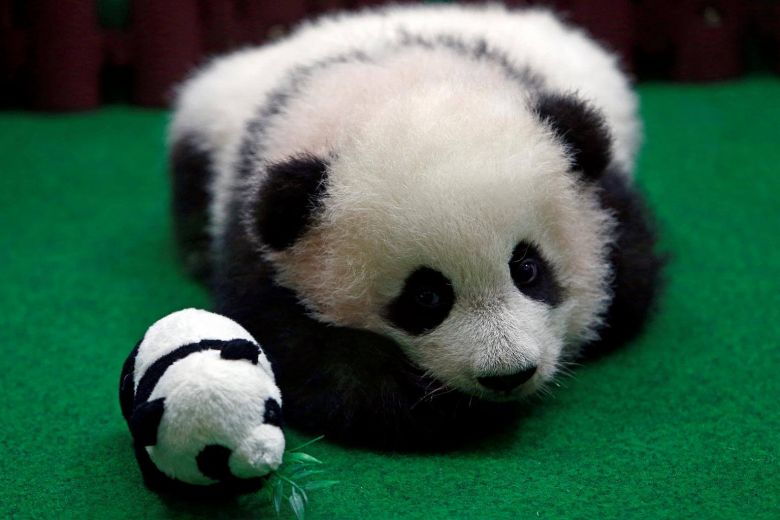
\includegraphics[width = \textwidth]{Figures/Panda_Cub}
	\caption{A newborn panda cub}
\end{figure}

\lipsum[3]

\begin{figure}[ht]
	\centering
	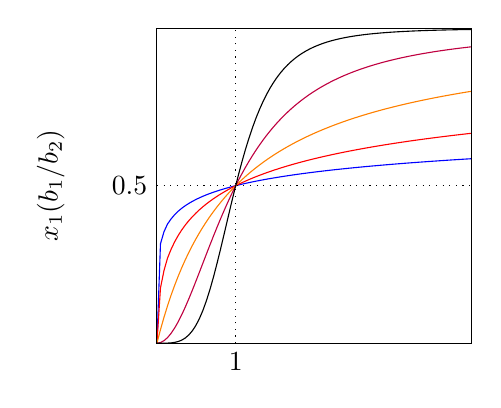
\begin{tikzpicture}[scale = 1]
	\foreach \a/\Col in {0.25/blue, 0.5/red, 1/orange, 2/purple, 4/black}
	{
		\draw[\Col] plot[domain = 0:4, variable = \x, samples = 90] ({\x}, {4 * (\a * \x^\a) / (\a + \a * \x^\a)});
	}
	\draw (0, 0) rectangle (4, 4);
	\draw [dotted] (1, 0) node[below]{$1$} -- (1, 4);
	\draw [dotted] (0, 2) node[left](p5){$0.5$} -- (4, 2);
	\node [left of= p5,rotate = 90]{$x_1(b_1/b_2)$};
\end{tikzpicture}

	\caption{Curves}
\end{figure}

\lipsum[4-5]

	\chapter{Frames}
\label{ch:ch2}

\epigraph{All human things are subject to decay, and when fate summons, Monarchs must obey.}{\textit{Mac Flecknoe} \\ \textsc{John Dryden}}

\begin{notice}
	It is a non-split frame\tablefootnote{This is a footnote in the frame.}.
\end{notice}

\begin{notice}
	\lipsum[6-7]
\end{notice}

\lipsum[8-9]

\begin{highlight}[Problem 1]
	It is a non-split frame\tablefootnote{This is a footnote in the frame, again.}.
\end{highlight}

\lipsum[10-11]

\begin{highlight}[Problem 2]
	\lipsum[12-13]
\end{highlight}

\begin{highlight*}[No Problem]
	\lipsum[14-15]
\end{highlight*}


	% The back matter.
	\backmatterpagestyle
	\bibliography{Back_Matter/Bibliography}
	\bookmarksetupnext{level = part} % `part` is `-1`.
	\appendix
	\begin{appendices}
		\chapter{Continued Fraction I}
\label{ap:confracI}

\lipsum[16]

\begin{equation*}
	x = a_0 + \frac{1}{\displaystyle a_1 
		+ \frac{1}{\displaystyle a_2 
			+ \frac{1}{\displaystyle a_3 + a_4}}}
\end{equation*}
		\chapter{Continued Fraction II}
\label{ap:confracII}

\lipsum[14]

\begin{equation*}
	x = a_0 + \frac{1}{a_1 + \frac{1}{a_2 + \frac{1}{a_3 + a_4}}}
\end{equation*}

	\end{appendices}
\end{document}